\subsection{SSD}
\label{SSD}

Herefter begynder artefakterne at komme tættere på koden. Ud fra Use Casesene opbygget i afsnit \ref{UseCases} kan vi oprette en SSD for hver use case. Dette hjælper med at give en forståelse for hvordan man vil implementere use casene kodemæssigt, f.eks ved hvilke input der kræves af brugerne. Sammen med SOC'en får vi en bedre ide for hvordan koden vil fungere, før vi overhovedet har skrevet en linje.

\begin{figure}[H]
    \caption{SSD for Book Ny Aftale}
    \centering
        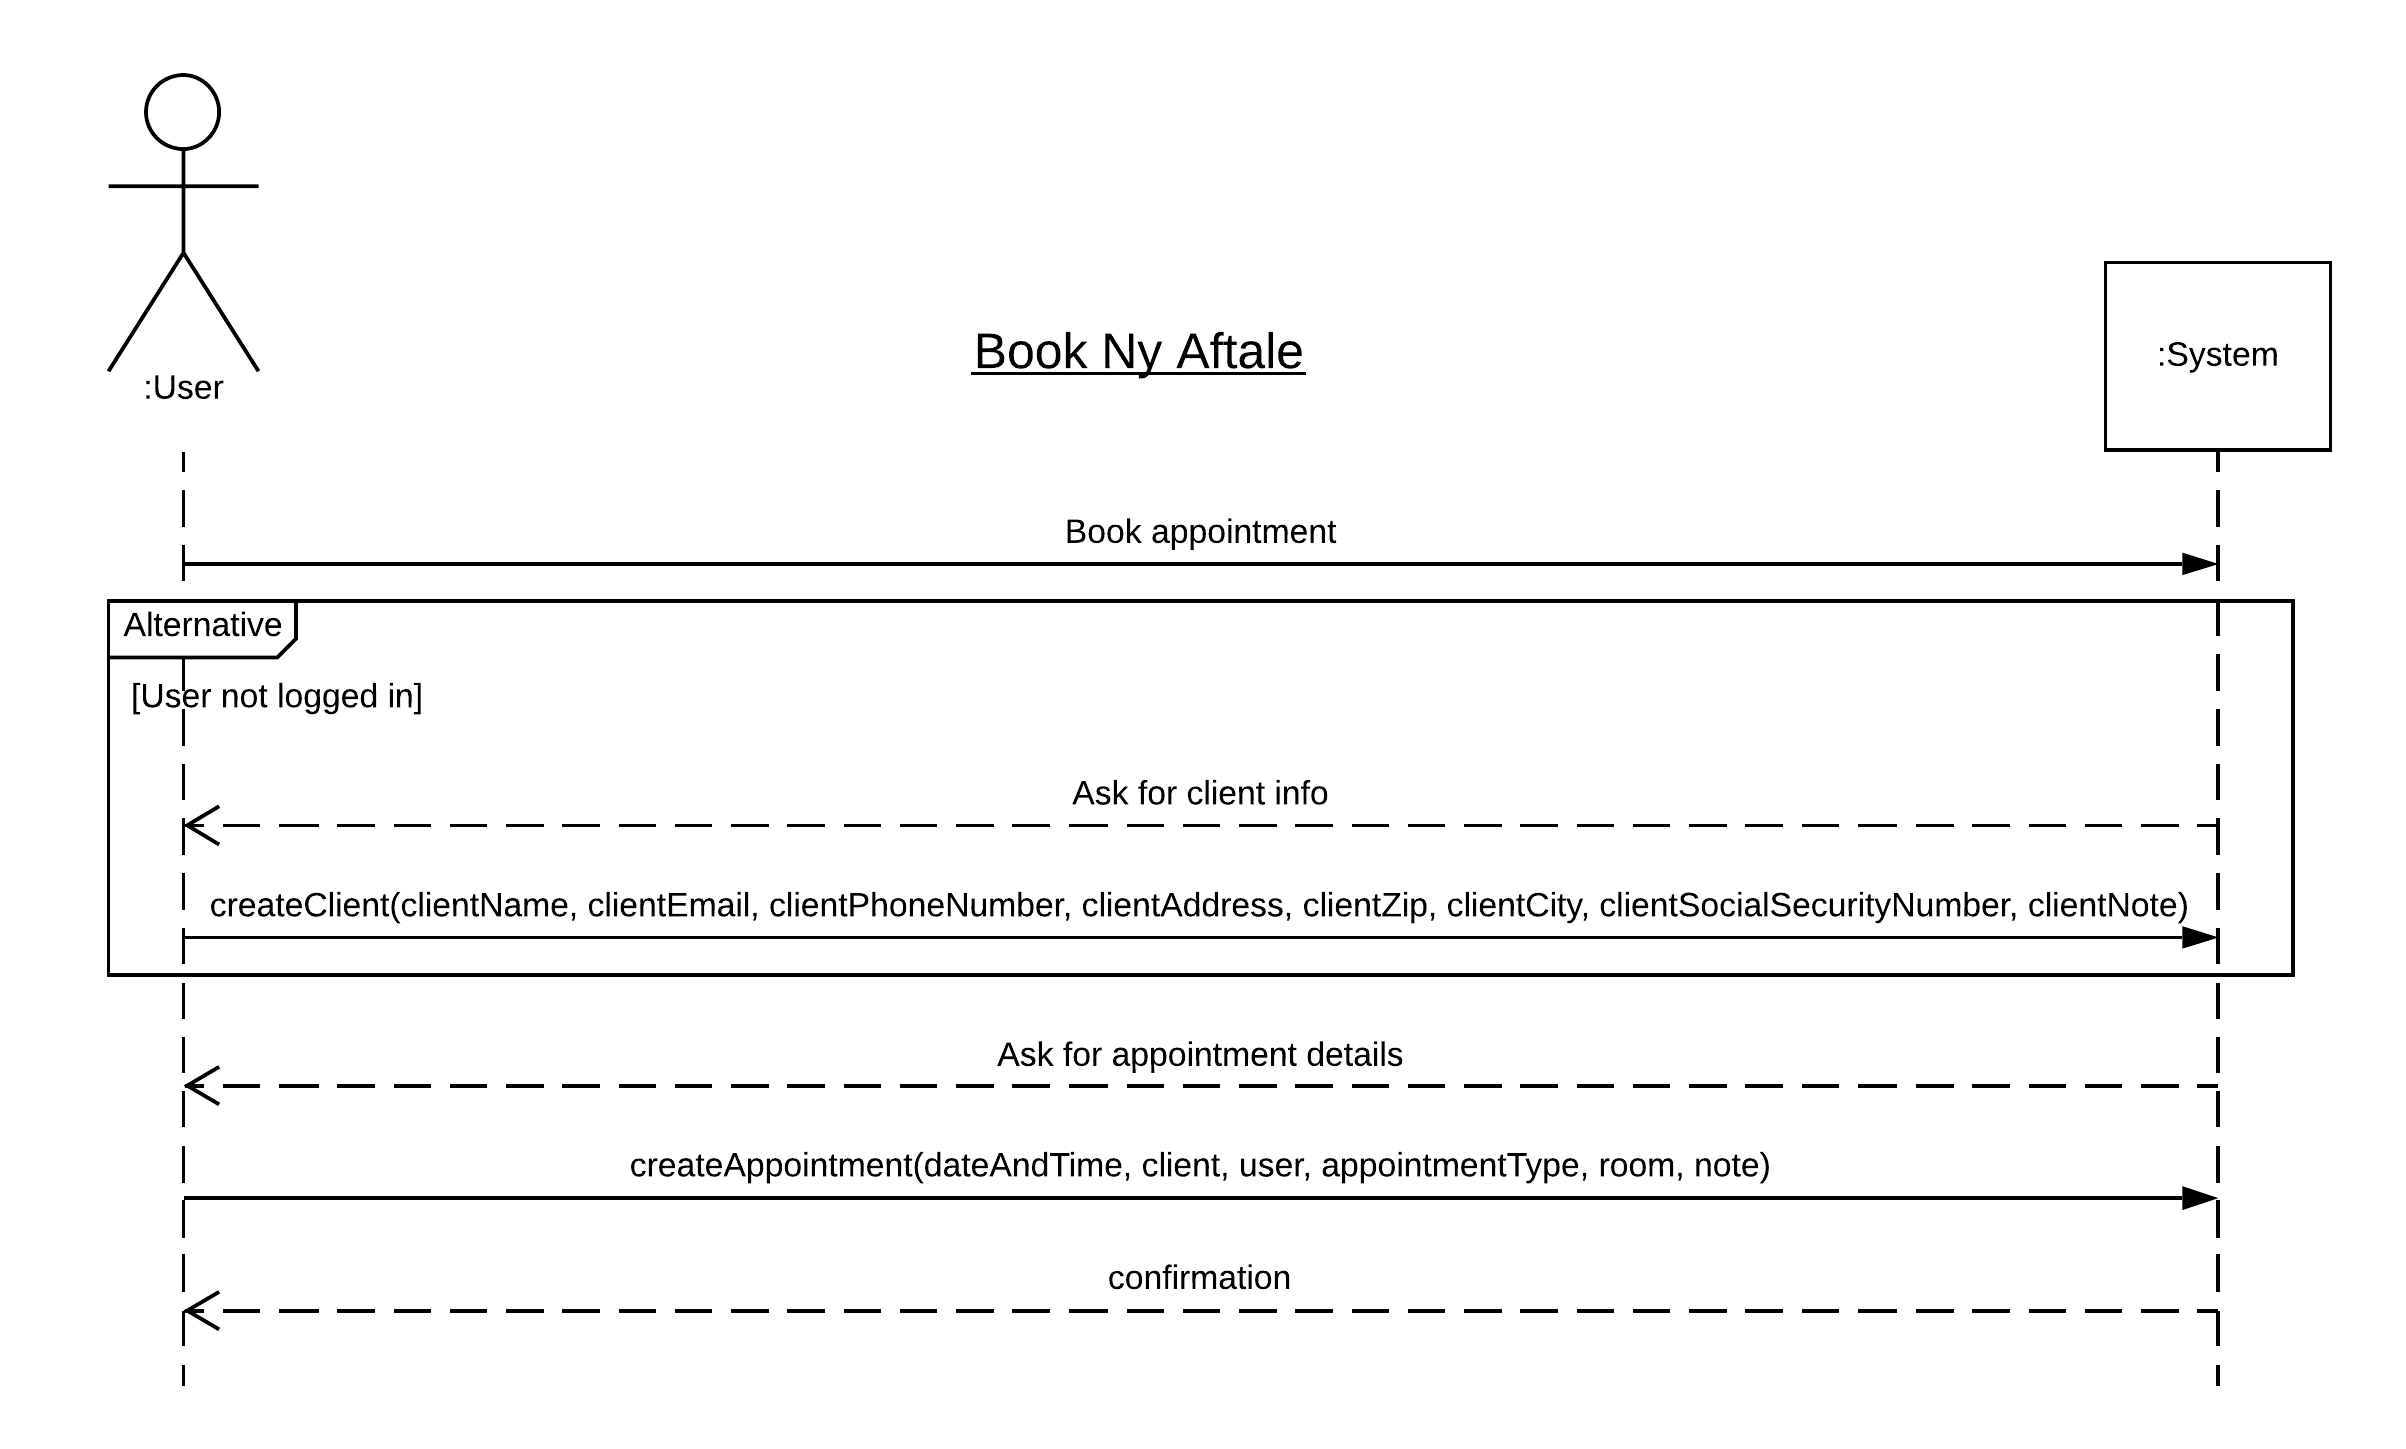
\includegraphics[width=\textwidth]{SSD.png}
    \label{forretning:ssd}
\end{figure}